\documentclass[aspectratio=169,10pt]{beamer}

\usetheme{default}
\usecolortheme{default}
\usefonttheme{professionalfonts}
\usepackage[T1]{fontenc}
\usepackage{ebgaramond}
\usepackage[scale=0.94]{tgheros}
\usepackage{amsmath,amssymb,mathtools,booktabs,graphicx,tikz}
\usetikzlibrary{arrows.meta,calc,positioning}
\usepackage[backend=biber,style=numeric,sorting=none,maxbibnames=3]{biblatex}
\addbibresource{references.bib}

% The official 2025 DLSU Brand Kit specifies Garamond for presentation titles
% and Frutiger for subtitles/headings.  EB Garamond and TeX Gyre Heros are the
% redistributable TeX substitutes used here; see README.md for access details.
\definecolor{dlsugreen}{RGB}{0,129,77}
\definecolor{dlsudarkgreen}{RGB}{0,82,49}
\definecolor{dlsupalegreen}{RGB}{235,246,240}
\definecolor{dlsucharcoal}{RGB}{34,43,46}
\definecolor{dlsumidgray}{RGB}{96,108,111}
\definecolor{dlsulightgray}{RGB}{244,246,245}
\definecolor{prospectivered}{RGB}{166,27,41}
\definecolor{resultblue}{RGB}{31,86,135}
\definecolor{protocolgray}{RGB}{245,247,249}
\definecolor{previeworange}{RGB}{181,96,0}

\setbeamercolor{normal text}{fg=dlsucharcoal,bg=white}
\setbeamercolor{structure}{fg=dlsugreen}
\setbeamercolor{alerted text}{fg=prospectivered}
\setbeamercolor{frametitle}{fg=dlsudarkgreen,bg=white}
\setbeamercolor{frametitle rule}{bg=dlsugreen}
\setbeamercolor{title}{fg=white}
\setbeamercolor{subtitle}{fg=white!88}
\setbeamercolor{author}{fg=white}
\setbeamercolor{institute}{fg=white!88}
\setbeamercolor{date}{fg=white!78}
\setbeamercolor{block title}{fg=white,bg=dlsugreen}
\setbeamercolor{block body}{fg=dlsucharcoal,bg=dlsupalegreen}
\setbeamercolor{block title alerted}{fg=white,bg=prospectivered}
\setbeamercolor{block body alerted}{fg=dlsucharcoal,bg=prospectivered!7}
\setbeamercolor{block title example}{fg=white,bg=resultblue}
\setbeamercolor{block body example}{fg=dlsucharcoal,bg=resultblue!7}
\setbeamercolor{itemize item}{fg=dlsugreen}
\setbeamercolor{itemize subitem}{fg=dlsugreen}
\setbeamercolor{enumerate item}{fg=dlsugreen}
\setbeamercolor{bibliography entry author}{fg=dlsucharcoal}
\setbeamercolor{bibliography entry title}{fg=dlsudarkgreen}
\setbeamercolor{bibliography entry location}{fg=dlsumidgray}
\setbeamercolor{bibliography entry note}{fg=dlsumidgray}
\setbeamercolor{author in head/foot}{fg=dlsumidgray,bg=white}
\setbeamercolor{date in head/foot}{fg=white,bg=dlsugreen}

\setbeamerfont{title}{family=\rmfamily,series=\bfseries,size=\fontsize{25}{28}}
\setbeamerfont{subtitle}{family=\sffamily,series=\bfseries,size=\fontsize{12.5}{15}}
\setbeamerfont{author}{family=\sffamily,series=\bfseries,size=\normalsize}
\setbeamerfont{institute}{family=\sffamily,size=\small}
\setbeamerfont{date}{family=\sffamily,size=\footnotesize}
\setbeamerfont{frametitle}{family=\sffamily,series=\bfseries,size=\fontsize{15.5}{18}}
\setbeamerfont{block title}{family=\sffamily,series=\bfseries}
\setbeamerfont{footline}{family=\sffamily,size=\fontsize{6.8}{8}}

\setbeamertemplate{navigation symbols}{}
\setbeamertemplate{blocks}[rounded][shadow=false]
\setbeamertemplate{itemize item}{\raise0.15ex\hbox{\small\textbullet}}
\setbeamertemplate{itemize subitem}{\raise0.15ex\hbox{\scriptsize\textbullet}}
\setbeamertemplate{enumerate item}{\insertenumlabel.}
\setbeamersize{text margin left=0.55cm,text margin right=0.55cm}

\setbeamertemplate{frametitle}{%
  \nointerlineskip
  \begin{beamercolorbox}[wd=\paperwidth,ht=0.64cm,dp=0.18cm,leftskip=0.55cm,rightskip=0.45cm]{frametitle}
    \usebeamerfont{frametitle}\insertframetitle
  \end{beamercolorbox}%
  \begin{beamercolorbox}[wd=\paperwidth,ht=0.035cm]{frametitle rule}\end{beamercolorbox}%
}

\setbeamertemplate{footline}{%
  \leavevmode
  \hbox{%
    \begin{beamercolorbox}[wd=.84\paperwidth,ht=2.8ex,dp=1.15ex,leftskip=.45cm,rightskip=.2cm]{author in head/foot}%
      \textbf{\textcolor{dlsugreen}{DE LA SALLE UNIVERSITY}}%
      \hspace{0.65em}\textcolor{dlsumidgray!55}{|}\hspace{0.65em}\insertshorttitle
    \end{beamercolorbox}%
    \begin{beamercolorbox}[wd=.16\paperwidth,ht=2.8ex,dp=1.15ex,center]{date in head/foot}%
      \insertframenumber\,/\,\inserttotalframenumber
    \end{beamercolorbox}%
  }%
}

\setbeamertemplate{title page}{%
  \vbox{}
  \vfill
  
\includegraphics[width=.34\paperwidth]{assets/dlsu-wordmark-white.png}\par
  \vspace{0.9em}
  {\usebeamerfont{title}\usebeamercolor[fg]{title}\inserttitle\par}
  \vspace{0.55em}
  {\color{white!55}\rule{.18\paperwidth}{0.8pt}\par}
  \vspace{0.65em}
  {\usebeamerfont{subtitle}\usebeamercolor[fg]{subtitle}\insertsubtitle\par}
  \vspace{1.1em}
  {\usebeamerfont{author}\usebeamercolor[fg]{author}\insertauthor\par}
  \vspace{0.25em}
  {\usebeamerfont{institute}\usebeamercolor[fg]{institute}\insertinstitute\par}
  \vspace{0.75em}
  {\usebeamerfont{date}\usebeamercolor[fg]{date}\insertdate\par}
  \vfill
}

\hypersetup{colorlinks=true,linkcolor=dlsugreen,urlcolor=dlsugreen,citecolor=resultblue}

\newcommand{\future}[1]{\textcolor{prospectivered}{#1}}
\newcommand{\HW}{H^{W}}
\newcommand{\TW}{T^{W}}
\newcommand{\RW}{R^{W}}

\title[Spectral--operator compatibility]{Compatibility of Spectral and Operator Reductions\\of a First-Principles Silicon Hamiltonian}
\subtitle{A constrained multi-objective formulation with aligned-operator diagnostics}
\author{Eugene Joseph M. Ragasa}
\institute{Department of Physics\\De La Salle University, Manila, Philippines}
\date{ICMSEP 2026 working presentation}

\begin{document}

{
\setbeamercolor{background canvas}{bg=dlsugreen}
\setbeamertemplate{footline}{}
\begin{frame}[plain]
  \titlepage
  \vspace{-0.9em}
  \begin{center}
    \scriptsize\color{white!84}
    Content-slide evidence: charcoal/blue.\qquad
    \textcolor{white}{Red: prospective work or an unexecuted extension.}
  \end{center}
\end{frame}
}

\begin{frame}{Long-term target: a substitutional-phosphorus operator}
  \small
  \begin{columns}[T]
    \column{0.47\textwidth}
      \begin{block}{Host route}
        \centering
        periodic DFT: Si
        $\longrightarrow$
        selected Bloch subspace
        $\longrightarrow$
        Wannier frame
        \[
          \{H^{W,\mathrm{Si}}(\mathbf R)\}.
        \]
      \end{block}
    \column{0.47\textwidth}
      \begin{block}{Impurity route}
        \centering
        periodic DFT: Si:P
        $\longrightarrow$
        selected Bloch subspace
        $\longrightarrow$
        Wannier frame
        \[
          \{H^{W,\mathrm{Si:P}}(\mathbf R)\}.
        \]
      \end{block}
  \end{columns}

  \begin{center}
    \textbf{Reconcile supercell, rank, subspace, orbital ordering, geometry,
    energy zero, units, and gauge}
    \[
      \Delta H_P^W(\mathbf R)
      =\widetilde H^{W,\mathrm{Si:P}}(\mathbf R)
       -\widetilde H^{W,\mathrm{Si}}(\mathbf R).
    \]
  \end{center}

  \begin{block}{Reduced-model target}
    \[
      H_{\mathrm{model}}^W
      =H_{\mathrm{host}}^W+\Delta H_P^W,
    \]
    followed by withheld checks against the aligned Si:P calculation before any
    finite-range compression is accepted.
  \end{block}

  \centering
  \future{ICMSEP scope: establish a compatible bulk-Si reference. The production Si:P
  calculation and authenticated impurity perturbation are subsequent prospective work;
  the current silicon evidence is a bounded tutorial control.}
\end{frame}

\begin{frame}{Can the operator be extracted in any frame? Yes, covariantly}
  \small
  \begin{block}{Fixed selected subspace and one common frame}
    For any periodic unitary $V(\mathbf k)$ applied to both represented systems,
    \begin{align*}
      H_X^{V}(\mathbf k)&=V^\dagger(\mathbf k)H_X(\mathbf k)V(\mathbf k),\\
      \Delta H_P^{V}(\mathbf k)&=V^\dagger(\mathbf k)\Delta H_P(\mathbf k)V(\mathbf k).
    \end{align*}
    The spectra and abstract operator difference are unchanged. The matrix entries and
    their distribution among real-space blocks change covariantly.
  \end{block}

  \begin{center}
    \Large
    one common frame
    $\Longrightarrow$
    equivalent representations of one operator difference
  \end{center}

  \begin{block}{Additional locality condition}
    A smooth periodic $V(\mathbf k)$ is needed for a localized Wannier representation.
    A discontinuous or rapidly varying gauge is algebraically valid but can produce
    long-ranged blocks.
  \end{block}
\end{frame}

\begin{frame}{Can independently chosen frames be subtracted? No}
  \begin{alertblock}{Independent coordinate arrays cannot be subtracted directly}
    \[
      V_P^\dagger H_{\mathrm{Si:P}}V_P
      -V_0^\dagger H_{\mathrm{Si}}V_0
    \]
    has no common-coordinate meaning unless an explicit, well-conditioned map identifies
    the two frames.
  \end{alertblock}

  \begin{columns}[T]
    \column{0.48\textwidth}
      \begin{block}{Gauge mismatch}
        Equal selected subspaces with a full-rank cross-overlap admit a unitary alignment.
        Phase, permutation, and internal unitary freedom can then be reconciled.
      \end{block}
    \column{0.48\textwidth}
      \begin{alertblock}{Subspace mismatch}
        Rank loss or unequal projectors is not removable by gauge alignment. The
        projection/disentanglement contract must be repaired or the residual reported.
      \end{alertblock}
  \end{columns}

  \vspace{0.5em}
  \centering
  For interpretable impurity blocks, prefer a shared projector-defined or host-anchored
  frame over two independently optimized MLWF gauges.
\end{frame}

\begin{frame}{Is the Kohn--Sham solution unique? Specify the object}
  \small
  \begin{tabular}{p{0.29\textwidth}p{0.62\textwidth}}
    \toprule
    Map or object & Qualified uniqueness statement\\
    \midrule
    $n_0\mapsto v_{\mathrm{ext}}$
      & Hohenberg--Kohn: unique up to an additive constant under the standard
        nondegenerate ground-state assumptions \cite{hohenberg1964}.\\[0.6em]
    $n_0\mapsto v_s$
      & The local KS potential is unique up to a constant when the density is
        noninteracting $v$-representable and the relevant uniqueness assumptions hold.\\[0.6em]
    $v_s\mapsto$ canonical KS states
      & Nondegenerate eigenstates are fixed only up to phase; degenerate eigenspaces admit
        unitary rotation.\\[0.6em]
    occupied projector $P\mapsto$ frame $F$
      & Never unique: $F$ and $FU$ represent the same projector for every unitary $U$.\\
    \bottomrule
  \end{tabular}

  \vspace{0.8em}
  \begin{alertblock}{The apparent contradiction}
    A density may determine a qualified local potential without determining a unique
    orbital frame. ``Invert the density to a potential'' and ``choose a basis inside an
    occupied or selected subspace'' are different inverse problems.
  \end{alertblock}
\end{frame}

\begin{frame}{Why orbital rotations can leave the density unchanged}
  \small
  Let $F(\mathbf k)$ collect equally occupied Bloch orbitals. Then
  \[
    P=FF^\dagger,
    \qquad F\mapsto FU,
    \qquad P\mapsto FUU^\dagger F^\dagger=P,
  \]
  and consequently
  \[
    n(\mathbf r)
      =\sum_{\mathbf k}\sum_{n\in\mathcal S}f_{\mathbf k}
       |\psi_{n\mathbf k}(\mathbf r)|^2
  \]
  is unchanged.

  \begin{block}{Wannier gauge freedom}
    The projector and equal-occupation density do not select an internal frame. A smooth
    periodic $U(\mathbf k)$ selects localized Wannier representatives of the same
    subspace.
  \end{block}

  \begin{alertblock}{Restricted freedom}
    Mixing unequal occupations generally changes the density. Mixing nondegenerate
    eigenstates preserves the selected subspace, but the Hamiltonian becomes
    non-diagonal and the rotated orbitals are no longer individual KS eigenstates.
  \end{alertblock}
\end{frame}

\begin{frame}{Where information is retained, quotiented out, or discarded}
  \scriptsize
  \begin{tabular}{p{0.27\textwidth}p{0.31\textwidth}p{0.32\textwidth}}
    \toprule
    Map & What remains & What is no longer explicit\\
    \midrule
    Many-body $\Psi\mapsto n$
      & Ground-state density
      & Correlations and phases; exact Hohenberg--Kohn theory gives conditional formal
        recovery, not an orbital gauge from the density alone \cite{hohenberg1964}\\[0.5em]
    KS frame $F\mapsto P=FF^\dagger$
      & Selected subspace and equal-occupation density
      & Internal unitary frame $U(\mathbf k)$\\[0.5em]
    Bloch matrix $H(\mathbf k)\mapsto\operatorname{spec}H(\mathbf k)$
      & Eigenvalues
      & Eigenvectors, projectors, orbital matrix structure, and hopping distribution\\[0.5em]
    $H(\mathbf k)\leftrightarrow\{T_{\mathbf R}\}$
      & Complete operator representation
      & Nothing in the complete transform; information is lost only by sampling,
        projection, or truncation\\
    \bottomrule
  \end{tabular}

  \vspace{0.35em}
  \begin{block}{Practical consequence}
    A wavefunction file retains one gauge-dependent representative $F(\mathbf k)$.
    Wannier construction uses those states and overlaps; the charge density alone is not
    sufficient to construct or align the desired tight-binding operator.
  \end{block}
\end{frame}

\begin{frame}{What physical change does the subtraction contain?}
  \small
  Let $\mathcal R_0$ be the pristine geometry, $\mathcal R_P$ the Si:P-relaxed
  positions, and $\widetilde H_X^W(\mathcal R)=\mathcal A_X[H_X^W(\mathcal R)]$ the
  Hamiltonian after declared state-space, energy-reference, and frame alignment.
  Two endpoint calculations give
  \[
    \Delta H_{P,\mathrm{total}}^W
      =\widetilde H_{\mathrm{Si:P}}^W(\mathcal R_P)
       -\widetilde H_{\mathrm{Si}}^W(\mathcal R_0),
  \]
  which generally combines substitution chemistry, self-consistent electronic
  screening, and structural relaxation.

  \begin{block}{A matched-geometry Si calculation separates two channels}
    \begin{align*}
      \Delta H_{P,\mathrm{chem}}^W
        &=\widetilde H_{\mathrm{Si:P}}^W(\mathcal R_P)
          -\widetilde H_{\mathrm{Si}}^W(\mathcal R_P),\\
      \Delta H_{P,\mathrm{relax}}^W
        &=\widetilde H_{\mathrm{Si}}^W(\mathcal R_P)
          -\widetilde H_{\mathrm{Si}}^W(\mathcal R_0),\\
      \Delta H_{P,\mathrm{total}}^W
        &=\Delta H_{P,\mathrm{chem}}^W+\Delta H_{P,\mathrm{relax}}^W.
    \end{align*}
  \end{block}

  \future{The production protocol must fix charge state, spin, supercell finite-size
  controls, structural branch, and whether the target is the screened Kohn--Sham
  perturbation or another effective operator.}
\end{frame}

\begin{frame}{Why four controls precede production subtraction}
  \begin{block}{Production question}
    What must be controlled before independently generated Si and Si:P DFT/Wannier
    operators can be aligned, subtracted, and compressed without confusing gauge,
    discretization, or model-reduction effects with the impurity response?
  \end{block}

  \begin{enumerate}
    \item \textbf{Exact 1-D rank-two benchmark:} isolates the gauge/locality mechanism
          and defines equal-accuracy range comparison.
    \item \textbf{2-D spectral-to-TB control:} tests multidimensional state spaces,
          Fourier conversion, mixed hoppings, and interpolation.
    \item \textbf{Rank-three multiband control:} tests pointwise versus restricted
          frame alignment and its locality consequences.
    \item \textbf{Silicon tutorial bridge:} tests same-frame operator decomposition and
          component-sensitive truncation on wavefunction-derived data.
  \end{enumerate}

  \vspace{0.4em}
  \centering
  $\{T_{\mathbf R}\}\ \longleftrightarrow\ H(\mathbf k)\
  \longrightarrow\ \operatorname{spec}H(\mathbf k)$

  \vspace{0.35em}
  \footnotesize
  Convention: $\mathbf k$ is the Bloch wave vector ($\hbar\mathbf k$ is crystal
  momentum); $\hat{\mathbf p}=-i\hbar\nabla$ is the canonical momentum operator.
\end{frame}

\begin{frame}{Why spectral targets are necessary but not sufficient}
  \centering
  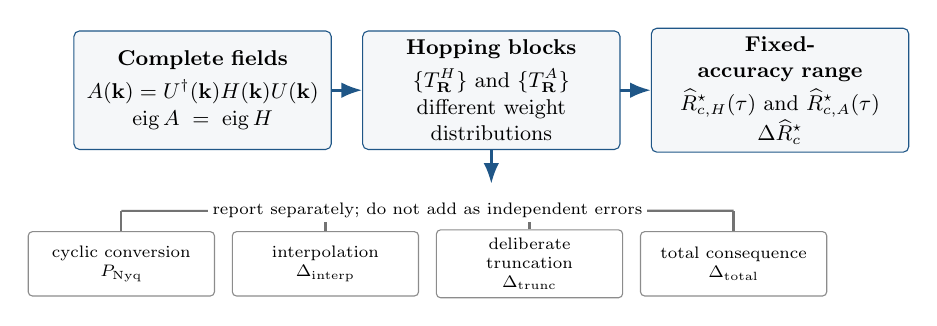
\begin{tikzpicture}[
    >=Latex,
    scale=0.86,transform shape,
    stage/.style={draw=resultblue,rounded corners=2pt,fill=protocolgray,
                  minimum width=3.8cm,minimum height=1.75cm,align=center,
                  font=\small,text width=3.45cm},
    channel/.style={draw=black!45,rounded corners=1.5pt,fill=white,
                    minimum width=2.75cm,minimum height=0.95cm,align=center,
                    font=\scriptsize,text width=2.45cm},
    arrow/.style={->,line width=1pt,resultblue},
    link/.style={line width=0.8pt,black!55}
  ]
    \node[stage] (complete) {
      \textbf{Complete fields}\\[1mm]
      $A(\mathbf k)=U^\dagger(\mathbf k)H(\mathbf k)U(\mathbf k)$\\
      $\operatorname{eig}A=\operatorname{eig}H$
    };
    \node[stage,right=0.45cm of complete] (fourier) {
      \textbf{Hopping blocks}\\[1mm]
      $\{T_{\mathbf R}^{H}\}$ and $\{T_{\mathbf R}^{A}\}$\\
      different weight distributions
    };
    \node[stage,right=0.45cm of fourier] (accuracy) {
      \textbf{Fixed-accuracy range}\\[1mm]
      $\widehat R_{c,H}^{\star}(\tau)$ and
      $\widehat R_{c,A}^{\star}(\tau)$\\
      $\Delta\widehat R_c^\star$
    };
    \draw[arrow] (complete) -- (fourier);
    \draw[arrow] (fourier) -- (accuracy);

    \node[channel,below=1.2cm of complete,xshift=-1.2cm] (conversion) {
      cyclic conversion\\$P_{\mathrm{Nyq}}$
    };
    \node[channel,right=0.25cm of conversion] (interpolation) {
      interpolation\\$\Delta_{\mathrm{interp}}$
    };
    \node[channel,right=0.25cm of interpolation] (truncation) {
      deliberate truncation\\$\Delta_{\mathrm{trunc}}$
    };
    \node[channel,right=0.25cm of truncation] (total) {
      total consequence\\$\Delta_{\mathrm{total}}$
    };
    \draw[link] (conversion.north) -- ++(0,0.30);
    \draw[link] (interpolation.north) -- ++(0,0.30);
    \draw[link] (truncation.north) -- ++(0,0.30);
    \draw[link] (total.north) -- ++(0,0.30);
    \draw[link] ($(conversion.north)+(0,0.30)$)
      -- ($(total.north)+(0,0.30)$);
    \draw[arrow] (fourier.south) -- ++(0,-0.50);
    \node[font=\scriptsize,fill=white,inner sep=2pt]
      at ($(interpolation.north)!0.5!(truncation.north)+(0,0.30)$)
      {report separately; do not add as independent errors};
  \end{tikzpicture}

  \vspace{0.35em}
  \scriptsize
  \textbf{G}: state-space and transport gates\quad
  \textbf{O}: representation/locality observables\quad
  \textbf{C}: approximation consequences\quad
  \textbf{V}: redundant verification of every arrow

  \vspace{0.25em}
  The benchmark isolates representation-induced locality from projection,
  discretization, and material-model errors; it does not replace physical spectral
  targets with diagnostic quantities.
\end{frame}

\begin{frame}{Bulk-Si reduction as a two-objective problem}
  \small
  For each declared tight-binding class $\mathcal M_j$, define two independent objectives
  \begin{align*}
    f_s(\theta)
      &=d_s\!\left(\mathbf s_\theta,\mathbf s_{\mathrm{DFT}}\right),\\
    f_o(\theta)
      &=d_o\!\left(H_\theta^W,H_{\mathrm{DFT}}^W\right),
  \end{align*}
  where $\mathbf s$ contains selected bands, gap, valley, and effective-mass observables,
  while $f_o$ compares aligned localized operators.

  \begin{block}{MOO problem within model class $\mathcal M_j$}
    \[
      \underset{\theta\in\mathcal M_j}{\operatorname{Pareto\!\!-minimize}}
      \quad \bigl(f_s(\theta),f_o(\theta)\bigr)
      \qquad\text{subject to qualification and model constraints.}
    \]
  \end{block}

  \begin{alertblock}{Do not hide the trade-off in one weighted score}
    A small weighted sum can compensate an unacceptable spectral error with a small
    operator error, or vice versa. The two objectives, their tolerances, and their Pareto
    trade-off remain visible.
  \end{alertblock}

  Gap isolation, overlap rank, sewing, Parseval, and verification checks are constraints
  or evidence about the calculation---not replacement objectives.
\end{frame}

\begin{frame}{Compatibility is a Pareto-feasibility question}
  \small
  \begin{columns}[T]
    \column{0.50\textwidth}
      \centering
      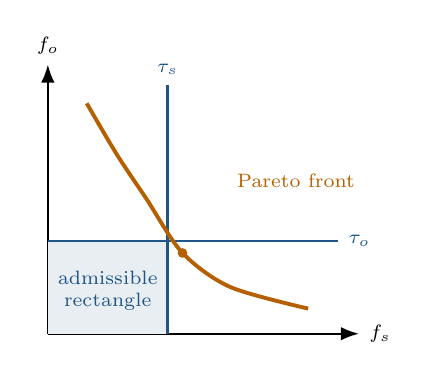
\begin{tikzpicture}[scale=0.76,>=Latex]
        \draw[->,line width=0.8pt] (0,0) -- (5.2,0)
          node[right,font=\scriptsize] {$f_s$};
        \draw[->,line width=0.8pt] (0,0) -- (0,4.5)
          node[above,font=\scriptsize] {$f_o$};
        \fill[resultblue!10] (0,0) rectangle (2.0,1.55);
        \draw[resultblue,line width=1pt] (2.0,0) -- (2.0,4.15)
          node[above,font=\scriptsize] {$\tau_s$};
        \draw[resultblue,line width=1pt] (0,1.55) -- (4.85,1.55)
          node[right,font=\scriptsize] {$\tau_o$};
        \draw[line width=1.4pt,previeworange]
          plot[smooth] coordinates {(0.65,3.85) (1.15,3.0) (1.65,2.25)
                                    (2.25,1.35) (3.05,0.78) (4.35,0.42)};
        \fill[previeworange] (2.25,1.35) circle (2.3pt);
        \node[font=\scriptsize,align=center,resultblue] at (1.0,0.72)
          {admissible\\rectangle};
        \node[font=\scriptsize,previeworange,anchor=west] at (3.0,2.55)
          {Pareto front};
      \end{tikzpicture}
    \column{0.46\textwidth}
      \scriptsize
      \begin{align*}
        \mathcal A_{s,j}&=\{\theta:f_s(\theta)\le\tau_s\},\\
        \mathcal A_{o,j}&=\{\theta:f_o(\theta)\le\tau_o\}.
      \end{align*}
      \begin{block}{Compatible class}
        \[
          \mathcal A_{s,j}\cap\mathcal A_{o,j}\neq\varnothing.
        \]
        A Pareto witness enters the admissible rectangle.
      \end{block}
      \begin{block}{Model selection}
        Choose the smallest reviewed class $j$ with a qualified common witness. Range or
        parameter count can be added as a declared third objective, but is not folded
        silently into $f_s$ or $f_o$.
      \end{block}
  \end{columns}

  \vspace{0.25em}
  \scriptsize
  If both admissible sets are nonempty but disjoint, report their normalized
  operator-space separation rather than a weighted compromise:
  $\delta_j^*=\inf_{\theta_s\in\mathcal A_{s,j},\theta_o\in\mathcal A_{o,j}}
  d_H(H_{\theta_s},H_{\theta_o})$.

  \future{The production bulk-Si Pareto front and compatibility witness remain
  uncomputed.}
\end{frame}

\begin{frame}{Paired diagnostic ledger for the mechanism schematic}
  \scriptsize
  \begin{tabular}{p{0.05\textwidth}p{0.20\textwidth}p{0.43\textwidth}p{0.19\textwidth}}
    \toprule
    Code & Schematic attachment & Diagnostic families & Interpretation\\
    \midrule
    \textbf{G}
      & complete fields and retained frame
      & external isolation gap; projector reconstruction; neighbor-overlap singular values;
        transport unitarity; reciprocal sewing and closure
      & must pass before observables are interpreted\\[0.7em]
    \textbf{O}
      & restricted alignment and hopping blocks
      & $\mu_{\max}$; irreducible operator residual; block Hermiticity; non-onsite and
        cumulative tail power
      & representation and locality observables\\[0.7em]
    \textbf{C}
      & four lower channel boxes and fixed-accuracy range
      & Nyquist conversion; interpolation; deliberate truncation; total Hamiltonian and
        spectral consequences; first passing range
      & separately named, nonadditive consequences\\[0.7em]
    \textbf{V}
      & every transformation arrow
      & Fourier nodal reconstruction; Parseval; Weyl bound; independent reconstruction;
        momentum/amplitude refinement
      & consistency evidence, not scientific acceptance\\
    \bottomrule
  \end{tabular}

  \vspace{0.35em}
  \begin{block}{Traceability rule}
    The schematic supplies the object-and-transformation map; the ledger supplies the
    gate, observable, consequence, or check attached to each element. Neither is complete
    without the other.
  \end{block}
\end{frame}

\begin{frame}{Diagnostic roles: do not collapse them into one score}
  \small
  \begin{columns}[T]
    \column{0.24\textwidth}
      \begin{alertblock}{Qualification gates}
        \begin{itemize}
          \item external isolation gap;
          \item overlap singular values;
          \item reciprocal sewing;
          \item Hermiticity.
        \end{itemize}
        Decide whether analysis may proceed.
      \end{alertblock}
    \column{0.24\textwidth}
      \begin{block}{Invariants}
        \begin{itemize}
          \item complete bands;
          \item projectors;
          \item Wilson-phase multisets;
          \item covariant reconstruction.
        \end{itemize}
        Establish equivalence under the declared map.
      \end{block}
    \column{0.24\textwidth}
      \begin{block}{Locality observables}
        \begin{itemize}
          \item block powers;
          \item omitted tails;
          \item spread estimators;
          \item shell counts.
        \end{itemize}
        Measure representation structure.
      \end{block}
    \column{0.24\textwidth}
      \begin{block}{Consequences}
        \begin{itemize}
          \item interpolation;
          \item truncation;
          \item total errors;
          \item Weyl/Parseval;
          \item independent reconstruction.
        \end{itemize}
        Quantify and verify approximation effects.
      \end{block}
  \end{columns}

  \vspace{0.4em}
  \centering
  A gate is not a convergence observable; omitted power is not a universal spectral
  bound; verification is not material validation.
\end{frame}

\begin{frame}{Reciprocal sewing is a diagnostic ladder, not one number}
  \small
  Let $S_{\mathbf G}(\mathbf k):\mathcal H_{\mathbf k}\rightarrow
  \mathcal H_{\mathbf k+\mathbf G}$ identify Bloch fibers across a reciprocal boundary.
  \begin{align*}
    H(\mathbf k+\mathbf G)S_{\mathbf G}&=S_{\mathbf G}H(\mathbf k),\\
    P(\mathbf k+\mathbf G)S_{\mathbf G}&=S_{\mathbf G}P(\mathbf k),\\
    F(\mathbf k+\mathbf G)&=S_{\mathbf G}F(\mathbf k)W_{\mathbf G}(\mathbf k),\\
    H_F(\mathbf k+\mathbf G)&=W_{\mathbf G}^\dagger
      H_F(\mathbf k)W_{\mathbf G}.
  \end{align*}
  \begin{tabular}{p{0.23\textwidth}p{0.66\textwidth}}
    \toprule
    Level & Required diagnostics\\
    \midrule
    Retained subspace & external isolation gap; constant rank; projector boundary covariance\\
    Neighbor transport & overlap singular values; full-rank gate; Procrustes residual\\
    Frame boundary & sewing-matrix unitarity; corrected endpoint discrepancy\\
    Closed paths & closure/holonomy phases and branch-cut proximity\\
    2-D/3-D extension & every primitive boundary; path consistency; plaquette closure;
      existence of one global periodic frame\\
    \bottomrule
  \end{tabular}

  \centering
  Wilson-loop and plaquette phases are sewing diagnostics here, not topological claims.
\end{frame}

\begin{frame}{1-D qualification and sewing: gates versus observations}
  \footnotesize
  \textit{$E_{\mathrm{ref}}$ is an arbitrary reference-energy normalization, not a band gap.}
  \vspace{-0.4em}

  \begin{tabular}{p{0.29\textwidth}p{0.25\textwidth}p{0.31\textwidth}}
    \toprule
    Diagnostic & Declared role or gate & Sampled observation\\
    \midrule
    External isolation gap $\min_q(\epsilon_3-\epsilon_2)/E_{\mathrm{ref}}$
      & must exceed $1.0$
      & minimum $1.0566461$\\[0.25em]
    Neighbor/closure overlap $\sigma_{\min}$
      & must exceed $0.99$; equality fails
      & minimum $0.9999989292$\\[0.25em]
    Neighbor Procrustes residual
      & conditioning record, not convergence observable
      & maximum $1.831\times10^{-3}$\\[0.25em]
    Transport-unitarity discrepancy
      & frame tolerance $10^{-10}$
      & maximum $1.89\times10^{-15}$\\[0.25em]
    Frame-orthonormality discrepancy
      & frame tolerance $10^{-10}$
      & maximum $3.34\times10^{-15}$\\[0.25em]
    Corrected periodic-closure discrepancy
      & numerical sewing check
      & maximum $9.55\times10^{-16}$\\[0.25em]
    Closure-holonomy phases
      & report ordered phase set; not a pass threshold
      & endpoint $(0.014181,0.018807)$ rad\\
    \bottomrule
  \end{tabular}

  \vspace{0.6em}
  \centering
  The gap and overlap thresholds are declared gates; $1.0566461$ and $0.9999989292$ are
  observed minima, not acceptance thresholds.
\end{frame}

\begin{frame}{From sewn operator to finite-range model}
  \small
  \begin{tabular}{p{0.21\textwidth}p{0.45\textwidth}p{0.24\textwidth}}
    \toprule
    Representation level & Diagnostic families & Scientific role\\
    \midrule
    Retained Bloch operator
      & frame isometry; projector lift; parent--retained reconstruction; complete spectra
      & establish the operator being represented\\[0.45em]
    Wannier/Fourier blocks
      & nodal round trip; Parseval; $T_{-\mathbf R}=T_{\mathbf R}^\dagger$;
        cyclic Nyquist power
      & verify conversion and ordinary-lattice structure\\[0.45em]
    Cross-representation alignment
      & pointwise covariant residual; one-global-unitary residual; symmetry intertwiners;
        cross-boundary sewing compatibility
      & separate gauge recovery from restricted comparison\\[0.45em]
    Locality
      & shell/block power; omitted power; spreads; tail norms; support-orbit closure
      & characterize representation, not spectral error\\[0.45em]
    Approximation consequences
      & separate interpolation, truncation, and total Hamiltonian max/RMS errors;
        separate sorted-band errors; Weyl check
      & quantify what compression changes\\[0.45em]
    Range decision
      & first passing sampled shell; predecessor failure; shifted evaluation and mesh
        refinement
      & equal-accuracy representation cost\\
    \bottomrule
  \end{tabular}
\end{frame}

\begin{frame}{1-D scientific observables: alignment and locality}
  \small
  \begin{align*}
    \mu_{\max}&=\frac{1}{\kappa}\max_{\phi} b_\phi,
    &
    L_{\mathrm{op},*}^2(s,\lambda)
      &=s^2+\kappa(\lambda-\mu_{\max})^2
        +\kappa(1-\mu_{\max}^2),\\
    \inf_{s\in\mathbb R,\lambda\ge0}L_{\mathrm{op},*}^2
      &=\kappa\!\left[1-\max(0,\mu_{\max})^2\right],
    &
    P_{>R_c}^{X}
      &=\frac{1}{2E_{\mathrm{ref}}^2}\sum_{|R|>R_c}\|T_R^X\|_F^2.
  \end{align*}
  \begin{tabular}{p{0.27\textwidth}p{0.62\textwidth}}
    \toprule
    Quantity & Interpretation\\
    \midrule
    $\mu_{\max}$
      & best continuously optimized global real-rotation correlation; an observable,
        not a transport gate\\[0.5em]
    irreducible operator residual
      & matrix information inaccessible to the restricted global alignment although the
        complete fields remain pointwise unitarily equivalent\\[0.5em]
    $P_{>0}^{X}$ and $P_{>R_c}^{X}$
      & non-onsite and cumulative omitted Frobenius power; locality diagnostics, not
        probabilities or universal spectral-error bounds\\[0.5em]
    sampled range $\widehat R_c^\star(\tau)$
      & first integer cutoff passing a separately named Hamiltonian or band criterion;
        the immediately preceding cutoff must fail\\
    \bottomrule
  \end{tabular}
\end{frame}

\begin{frame}{1-D consequence channels and redundant checks}
  \scriptsize
  \begin{tabular}{p{0.25\textwidth}p{0.42\textwidth}p{0.23\textwidth}}
    \toprule
    Channel/check & Compared objects & Sampled evidence\\
    \midrule
    Cyclic Nyquist conversion
      & normalized power in the removed $-N/2$ representative
      & $8.87\times10^{-32}$ to $1.14\times10^{-31}$\\[0.45em]
    Interpolation
      & finite interpolant versus direct field on disjoint mesh
      & max Hamiltonian $2.46\times10^{-14}$; band $2.35\times10^{-14}$\\[0.45em]
    Deliberate truncation
      & truncated ordinary-lattice field versus full interpolant
      & matrix and band max/RMS retained separately\\[0.45em]
    Total consequence
      & truncated field versus direct field
      & separate Hamiltonian and band cutoff decisions\\[0.45em]
    Truncation Parseval
      & squared RMS Hamiltonian error versus normalized omitted power
      & discrepancies $8.33\times10^{-17}$ and $1.11\times10^{-16}$\\[0.45em]
    Weyl check
      & max band error divided by its Frobenius bound
      & ratio $0.0087$ to $0.9984\le1$\\[0.45em]
    Momentum refinement
      & nested construction meshes plus shifted evaluation meshes
      & zero sampled cutoff-decision changes\\
    \bottomrule
  \end{tabular}

  \centering
  Conversion, interpolation, truncation, and total consequences are nonadditive channels.
\end{frame}

\begin{frame}{Material subtraction requires another diagnostic ladder}
  \scriptsize
  \begin{tabular}{p{0.20\textwidth}p{0.48\textwidth}p{0.22\textwidth}}
    \toprule
    Level & Diagnostics and gates & Present status\\
    \midrule
    DFT parents
      & structure and pseudopotential identity; SCF/cutoff/$\mathbf k$ convergence;
        complete target bands; symmetry and energy-reference conventions
      & \future{production pending}\\[0.35em]
    Wannier subspaces
      & projectability; windows; disentanglement; rank; centers/spreads; interpolation;
        reciprocal sewing and symmetry covariance
      & tutorial only\\[0.35em]
    Host--impurity identification
      & same supercell and orbital inventory; host lift; cross-overlap singular values;
        site/orbital matching; cross-system sewing and symmetry intertwiners
      & \future{unexecuted}\\[0.35em]
    Aligned subtraction
      & common energy zero and units; pointwise/common-frame residuals; Hermiticity;
        exact readdition $H_{\mathrm{Si}}^W+\Delta H_P^W=H_{\mathrm{Si:P}}^W$
      & \future{unexecuted}\\[0.35em]
    Physical decomposition
      & matched-geometry chemical and relaxation channels; charge/spin branch;
        supercell finite-size and far-field recovery
      & \future{open controls}\\[0.35em]
    Reduced impurity model
      & locality tails; symmetry-resolved blocks; truncation channels; withheld bands,
        valley, masses, and operator residuals
      & \future{unexecuted}\\[0.35em]
    Evidence identity
      & inputs, executable, pseudopotentials, source revision, checksums, verifier, and
        immutable evidence boundary
      & \future{production pending}\\
    \bottomrule
  \end{tabular}

  \centering
  A later diagnostic cannot repair a failed state-space, sewing, or provenance gate.
\end{frame}

\begin{frame}{Comparison contract: align spaces before subtraction}
  \begin{columns}[T]
    \column{0.50\textwidth}
      \begin{block}{Parent and retained spaces}
        \[
          F(\mathbf k):\mathbb C^r\rightarrow\mathcal H_p,
          \qquad F^\dagger F=I_r,
        \]
        \[
          H_{\mathrm{ret}}(\mathbf k)
          =F^\dagger(\mathbf k)H_p(\mathbf k)F(\mathbf k).
        \]
        A parent-space comparison requires the projector $P=FF^\dagger$ and an explicit
        lift $F H_{\mathrm{ret}}F^\dagger$.
      \end{block}
    \column{0.46\textwidth}
      \begin{alertblock}{Subtraction is undefined unless we fix}
        \begin{itemize}
          \item rank and state-space map;
          \item basis and orbital ordering;
          \item gauge or admissible alignment;
          \item energy zero and units;
          \item lattice geometry and Fourier convention.
        \end{itemize}
      \end{alertblock}
  \end{columns}

  \vspace{0.5em}
  \centering
  An eigenvalue array is spectral data; it is not a Hamiltonian in orbital coordinates.
\end{frame}

\begin{frame}{Result 1 theory: exact rank-two geometry}
  Write the retained field as $H=\bar E I_2+D$ with $\operatorname{tr}D=0$, and consider
  the positive trace--traceless candidate
  \[
    C_{s,\lambda}=\bar E I_2+sE_{\mathrm{ref}}I_2+\lambda D,
    \qquad \lambda>0.
  \]
  Under the declared weighting and one global real rotation,
  \begin{align*}
    L_{\mathrm{spec}}^2(s,\lambda)
      &=s^2+\kappa(\lambda-1)^2,\\
    L_{\mathrm{op},*}^2(s,\lambda)
      &=s^2+\kappa(\lambda-\mu_{\max})^2
        +\kappa(1-\mu_{\max}^2).
  \end{align*}

  \begin{columns}[T]
    \column{0.48\textwidth}
      \begin{block}{Smooth flat parent}
        $\mu_{\max}(a)=J_0(2a)$ gives exact alignment-threshold laws.
      \end{block}
    \column{0.48\textwidth}
      \begin{block}{Exact locality identity}
        The irreducible squared matrix residual equals normalized Fourier power outside
        the onsite block.
      \end{block}
  \end{columns}
\end{frame}

\begin{frame}{Result 1 numerical outcome: equal-accuracy range inflation}
  \begin{columns}[T]
    \column{0.62\textwidth}
      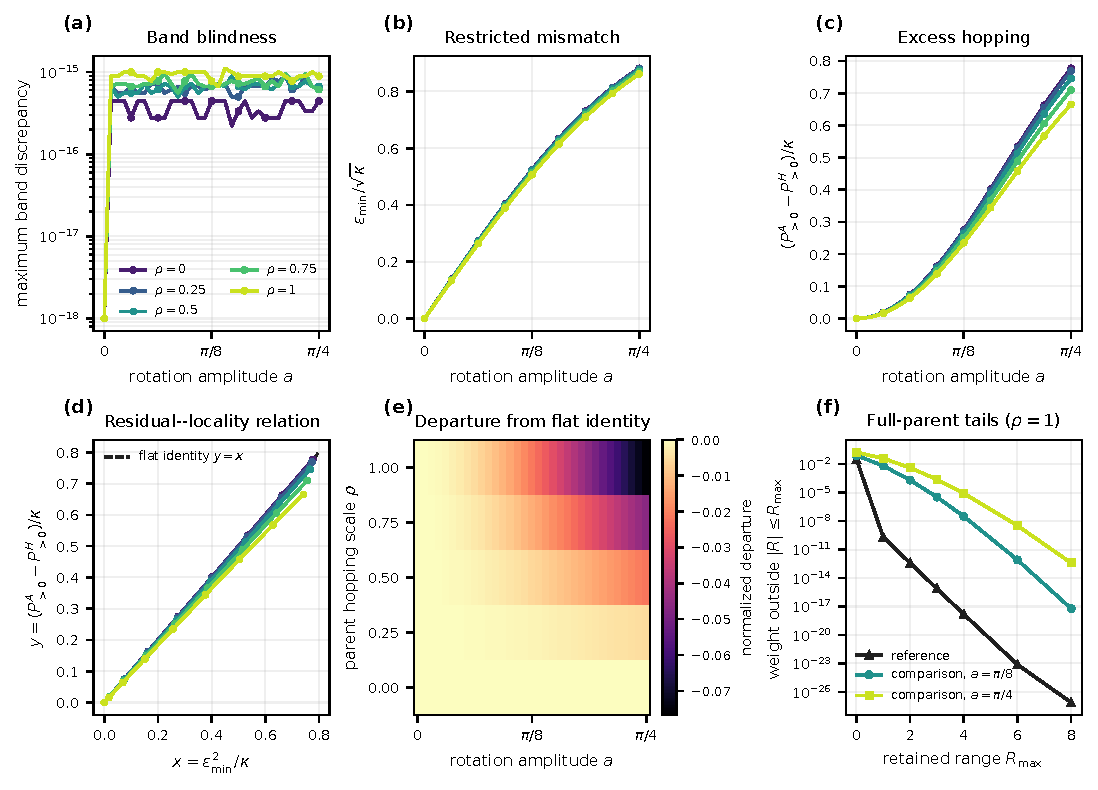
\includegraphics[width=\linewidth]{assets/band-equivalence-locality-scientific-story.pdf}
    \column{0.35\textwidth}
      \begin{itemize}
        \item Complete rank-two fields are related by a smooth $\mathbf k$-dependent
              $SO(2)$ rotation.
        \item Their bands agree pointwise.
        \item One global real rotation cannot recover the full gauge.
        \item At $\tau=10^{-8}E_{\mathrm{ref}}$:
      \end{itemize}
      \[
        \widehat R_{c,\mathrm{ref}}^\star=4,
        \qquad
        \widehat R_{c,\mathrm{comp}}^\star=10.
      \]
      \begin{alertblock}{Interpretation}
        $\Delta\widehat R_c^\star=6$ measures sampled representation cost, not physical
        inequivalence.
      \end{alertblock}
  \end{columns}
\end{frame}

\begin{frame}{Result 2 construction: spectral data to tight binding}
  For $d\in\{2,3\}$, keep four orbitals per cell and place the tensor structure in the
  lattice translations:
  \[
    \widehat K_{\rho,N}^{(d)}
    =I_{N^d}\otimes T_0+
      \frac{\rho}{d}\sum_{\alpha=1}^{d}
      \left(\mathsf S_{\alpha,N}\otimes T_+
      +\mathsf S_{\alpha,N}^\dagger\otimes T_-\right).
  \]
  \begin{center}
    \large
    cell--orbital operator
    $\xleftrightarrow{\ \mathcal F_{d,N}\ }$
    Bloch direct sum
    $\xleftrightarrow{\ Q(\mathbf k)\ }$
    complete eigensystem
  \end{center}
  \begin{center}
    \large
    $\xrightarrow{\ F(\mathbf k)\ }$
    retained Bloch field
    $\xleftrightarrow{\ \mathcal F_{d,N}^{-1}\ }$
    Wannier/TB blocks
  \end{center}

  \begin{alertblock}{Projection is not structural compression}
    Even a gapped finite-range parent can acquire infinite Fourier support after spectral
    projection because its projector need not be a finite Fourier polynomial.
  \end{alertblock}
\end{frame}

\begin{frame}{Result 2 evidence: reconstruction versus interpolation}
  \begin{columns}[T]
    \column{0.61\textwidth}
      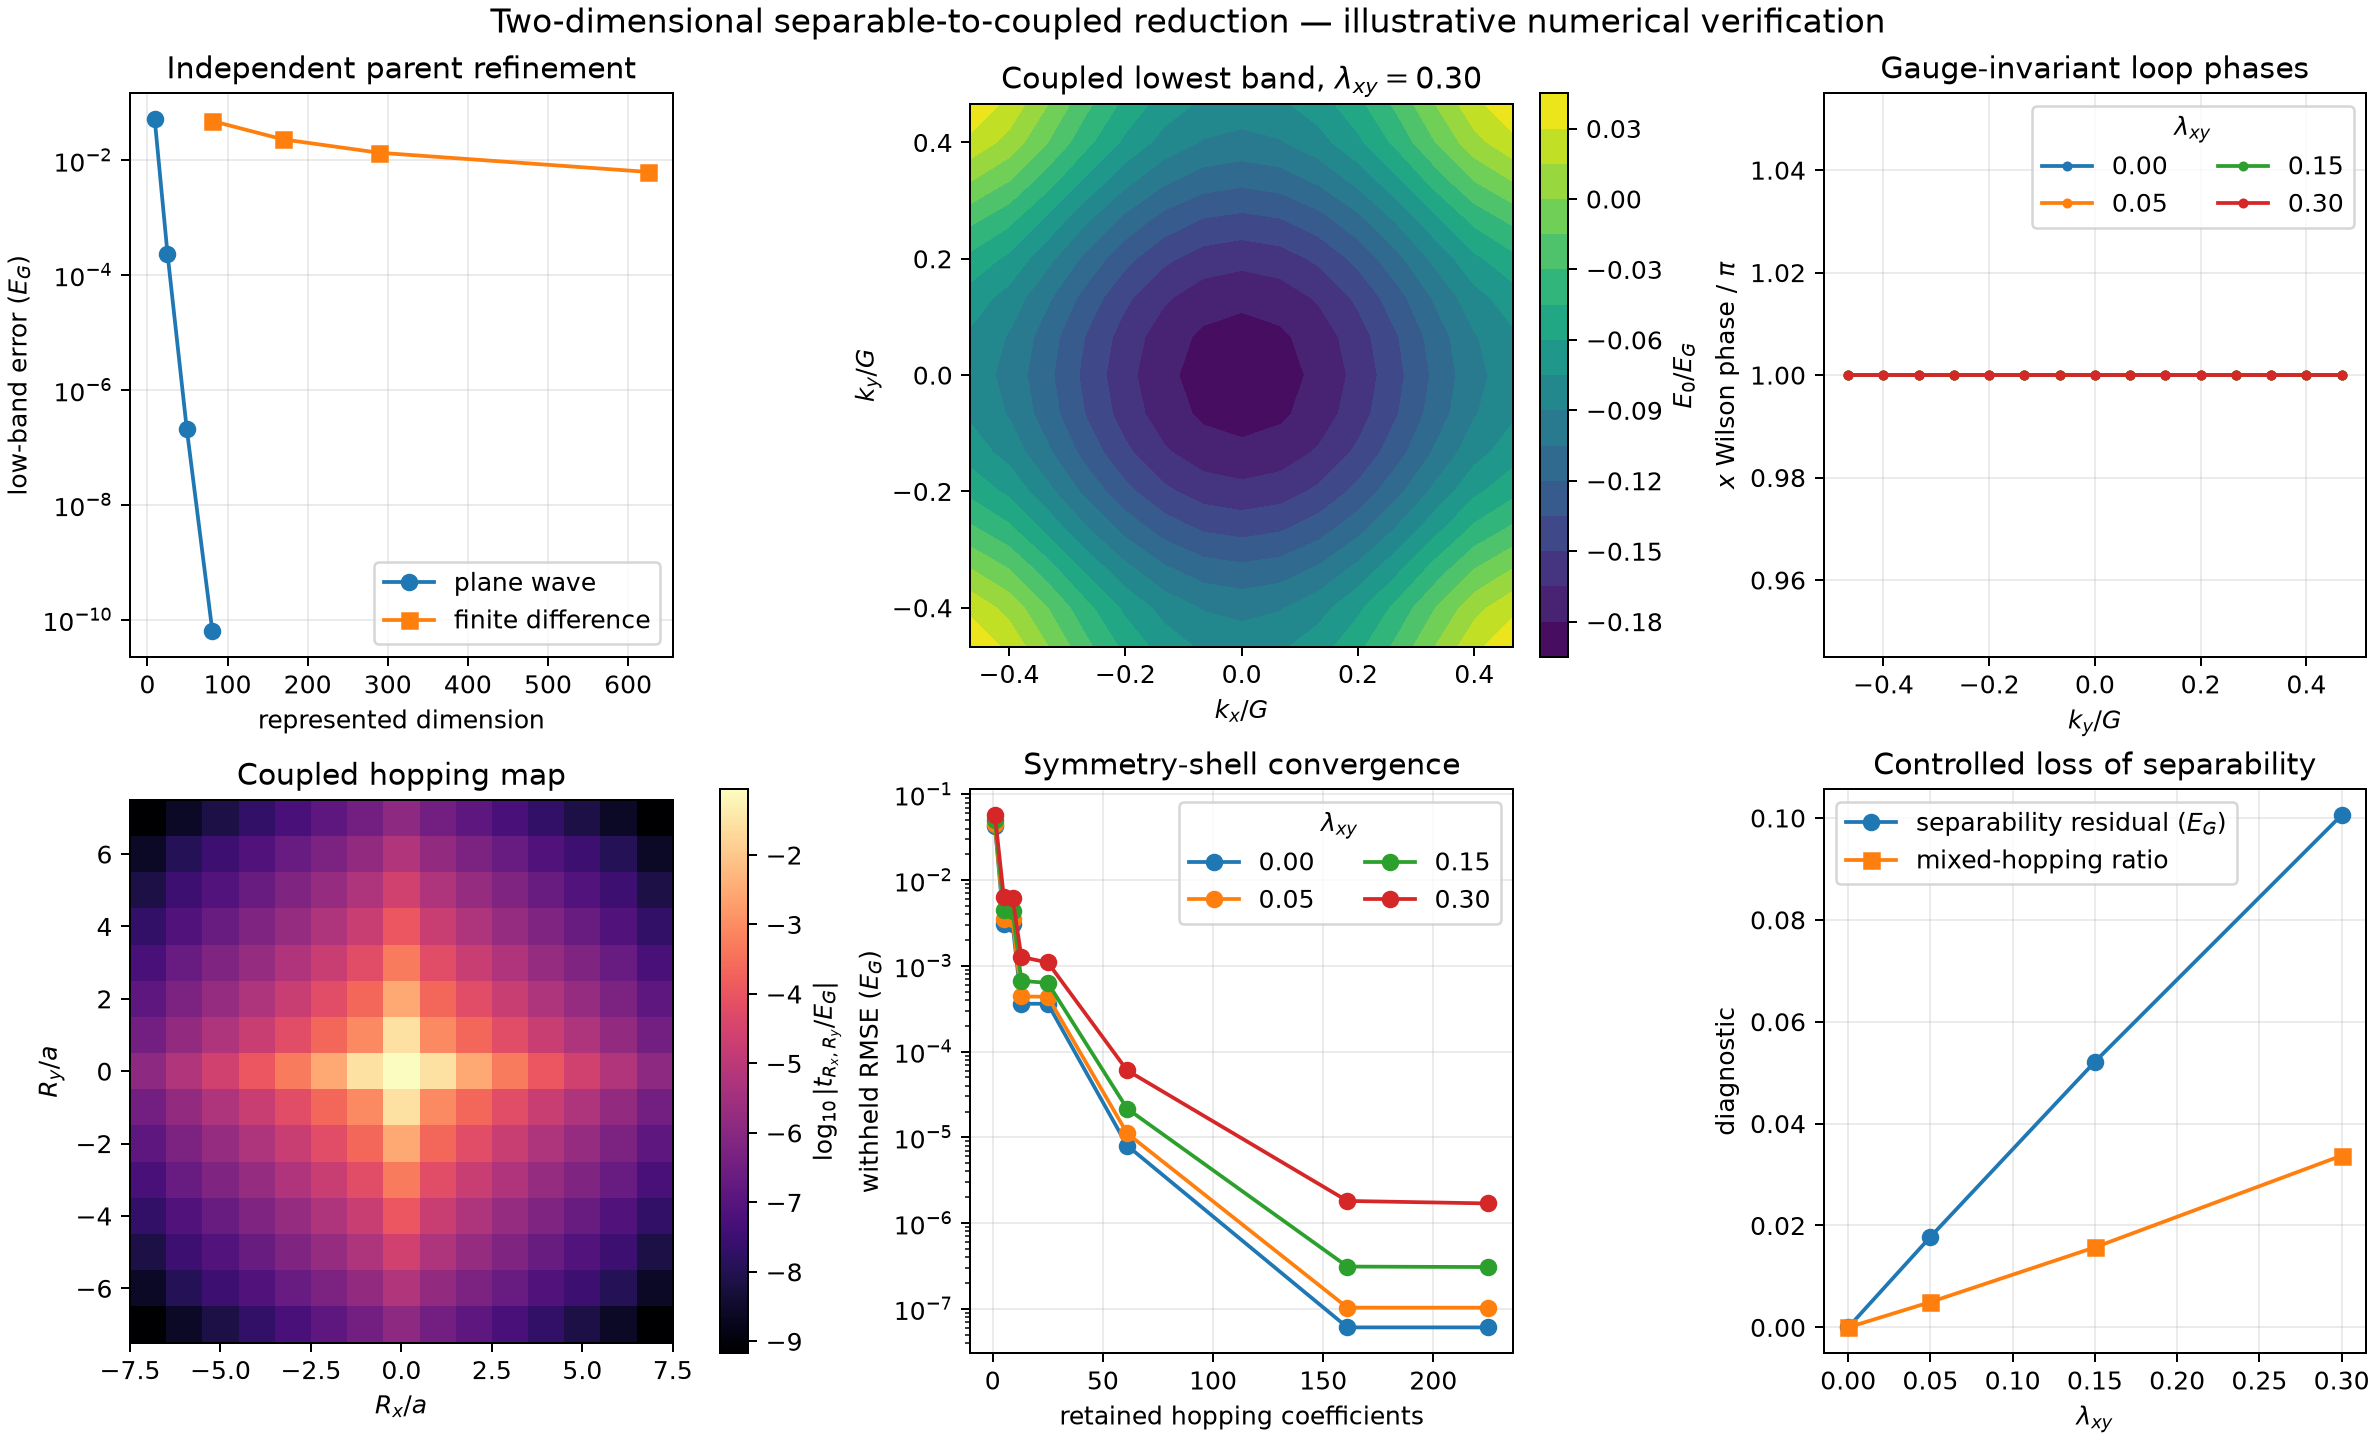
\includegraphics[width=\linewidth]{assets/periodic-2d-summary.png}
    \column{0.36\textwidth}
      \begin{itemize}
        \item At zero mixed coupling, the represented Kronecker-sum discrepancy is zero.
        \item Product-spectrum discrepancy:
              $3.55\times10^{-14}E_{\mathrm{ref}}$.
        \item At $\lambda_{xy}=0.30$, mixed-direction hopping norm:
              $1.94\times10^{-3}E_{\mathrm{ref}}$.
        \item Complete $15\times15$ transform reconstructs its nodes within
              $1.11\times10^{-15}E_{\mathrm{ref}}$.
        \item Independent $31\times31$ evaluation retains nonzero interpolation error.
      \end{itemize}
  \end{columns}

  \vspace{0.3em}
  \centering
  Exact sampled reconstruction $\neq$ off-node convergence.
\end{frame}

\begin{frame}{Result 3: pointwise and global unitary alignment}
  For equal-rank frames, form the cross-overlap
  \[
    M(\mathbf k)=F_{\mathrm{cand}}^\dagger(\mathbf k)
    F_{\mathrm{ref}}(\mathbf k)
    =L(\mathbf k)\Sigma(\mathbf k)V^\dagger(\mathbf k).
  \]
  \begin{columns}[T]
    \column{0.48\textwidth}
      \begin{block}{Pointwise family}
        \[
          U(\mathbf k)=L(\mathbf k)V^\dagger(\mathbf k).
        \]
        Align each $\mathbf k$ point before Fourier transformation. This can mix hopping ranges.
      \end{block}
    \column{0.48\textwidth}
      \begin{block}{One-global-unitary family}
        \[
          B=\sum_{\mathbf k}M(\mathbf k)=L_B\Sigma_BV_B^\dagger,
          \qquad U_{\mathrm{glob}}=L_BV_B^\dagger.
        \]
        One coordinate identification is used for the entire Brillouin zone.
      \end{block}
  \end{columns}

  \vspace{0.4em}
  These are different scientific restrictions, not two approximations to the same fit
  \cite{schonemann1966,higham1986}. Rank deficiency---including equality at the cutoff---
  fails closed.
\end{frame}

\begin{frame}{Result 3a: multiband gauge consistency does not fix locality}
  \begin{columns}[T]
    \column{0.62\textwidth}
      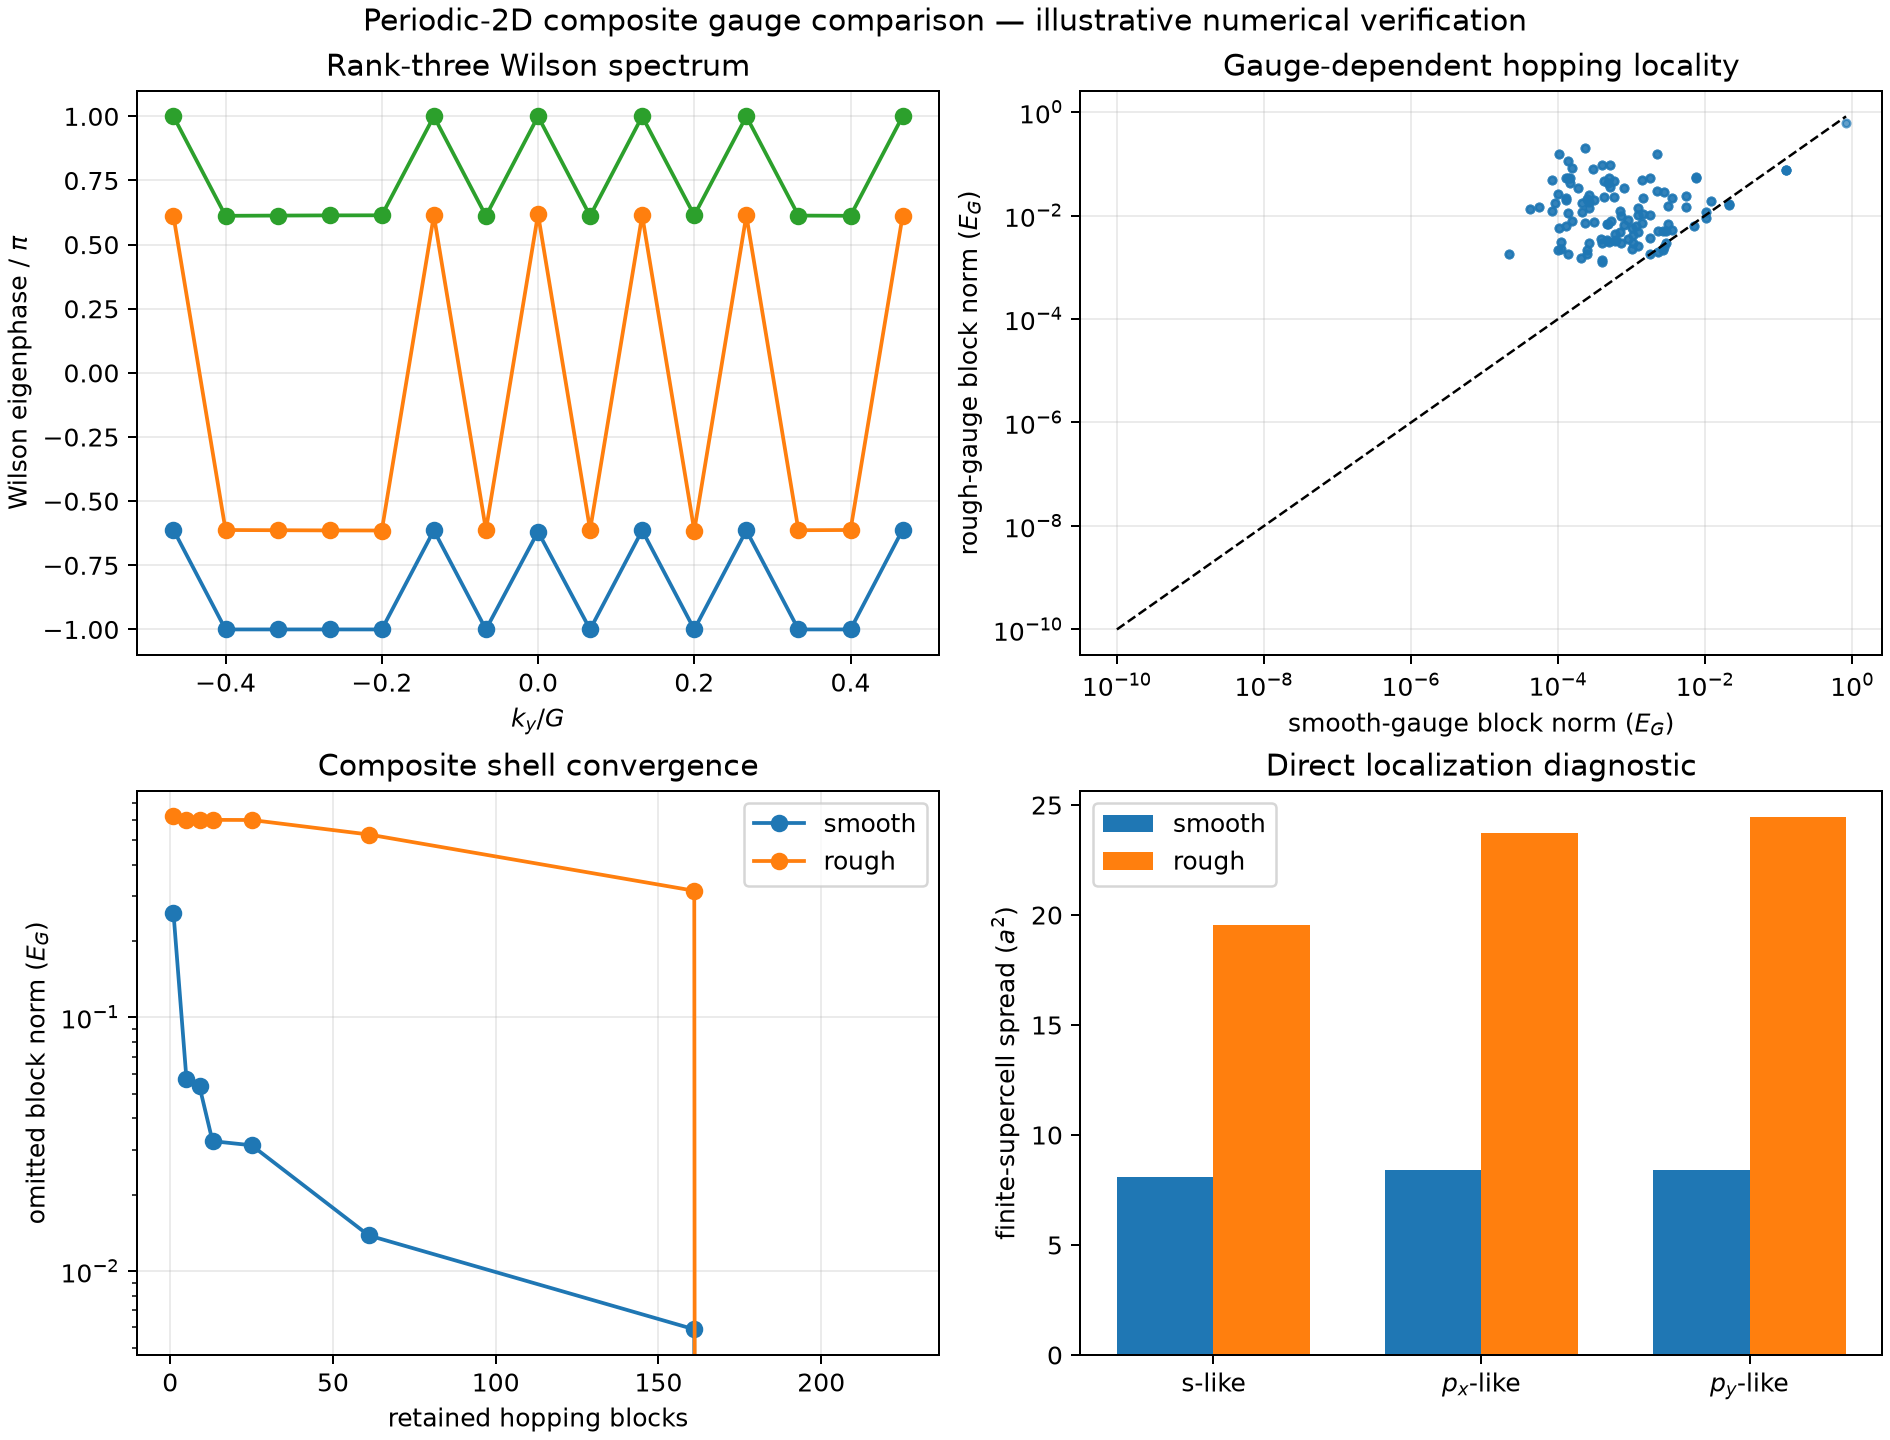
\includegraphics[width=\linewidth,height=0.55\textheight,keepaspectratio]{assets/periodic-2d-composite-summary.png}
    \column{0.35\textwidth}
      \begin{itemize}
        \item Lowest-three-band smooth and rough frames.
        \item Spectral agreement:
              $1.22\times10^{-15}E_{\mathrm{ref}}$.
        \item Wilson-phase multiset agreement:
              $2.22\times10^{-15}$.
        \item Common-grid spreads:
              $24.90a^2$ versus $67.70a^2$.
        \item Tail beyond squared-radius 18:
              $1.38\times10^{-2}E_{\mathrm{ref}}$ versus $5.25\times10^{-1}E_{\mathrm{ref}}$.
      \end{itemize}
  \end{columns}

  \vspace{0.2em}
  \centering
  Wilson phases are sewing diagnostics here, not a continuum topological claim.
\end{frame}

\begin{frame}{Result 3b: one algorithm-selected Wannier90 frame}
  \begin{columns}[T]
    \column{0.60\textwidth}
      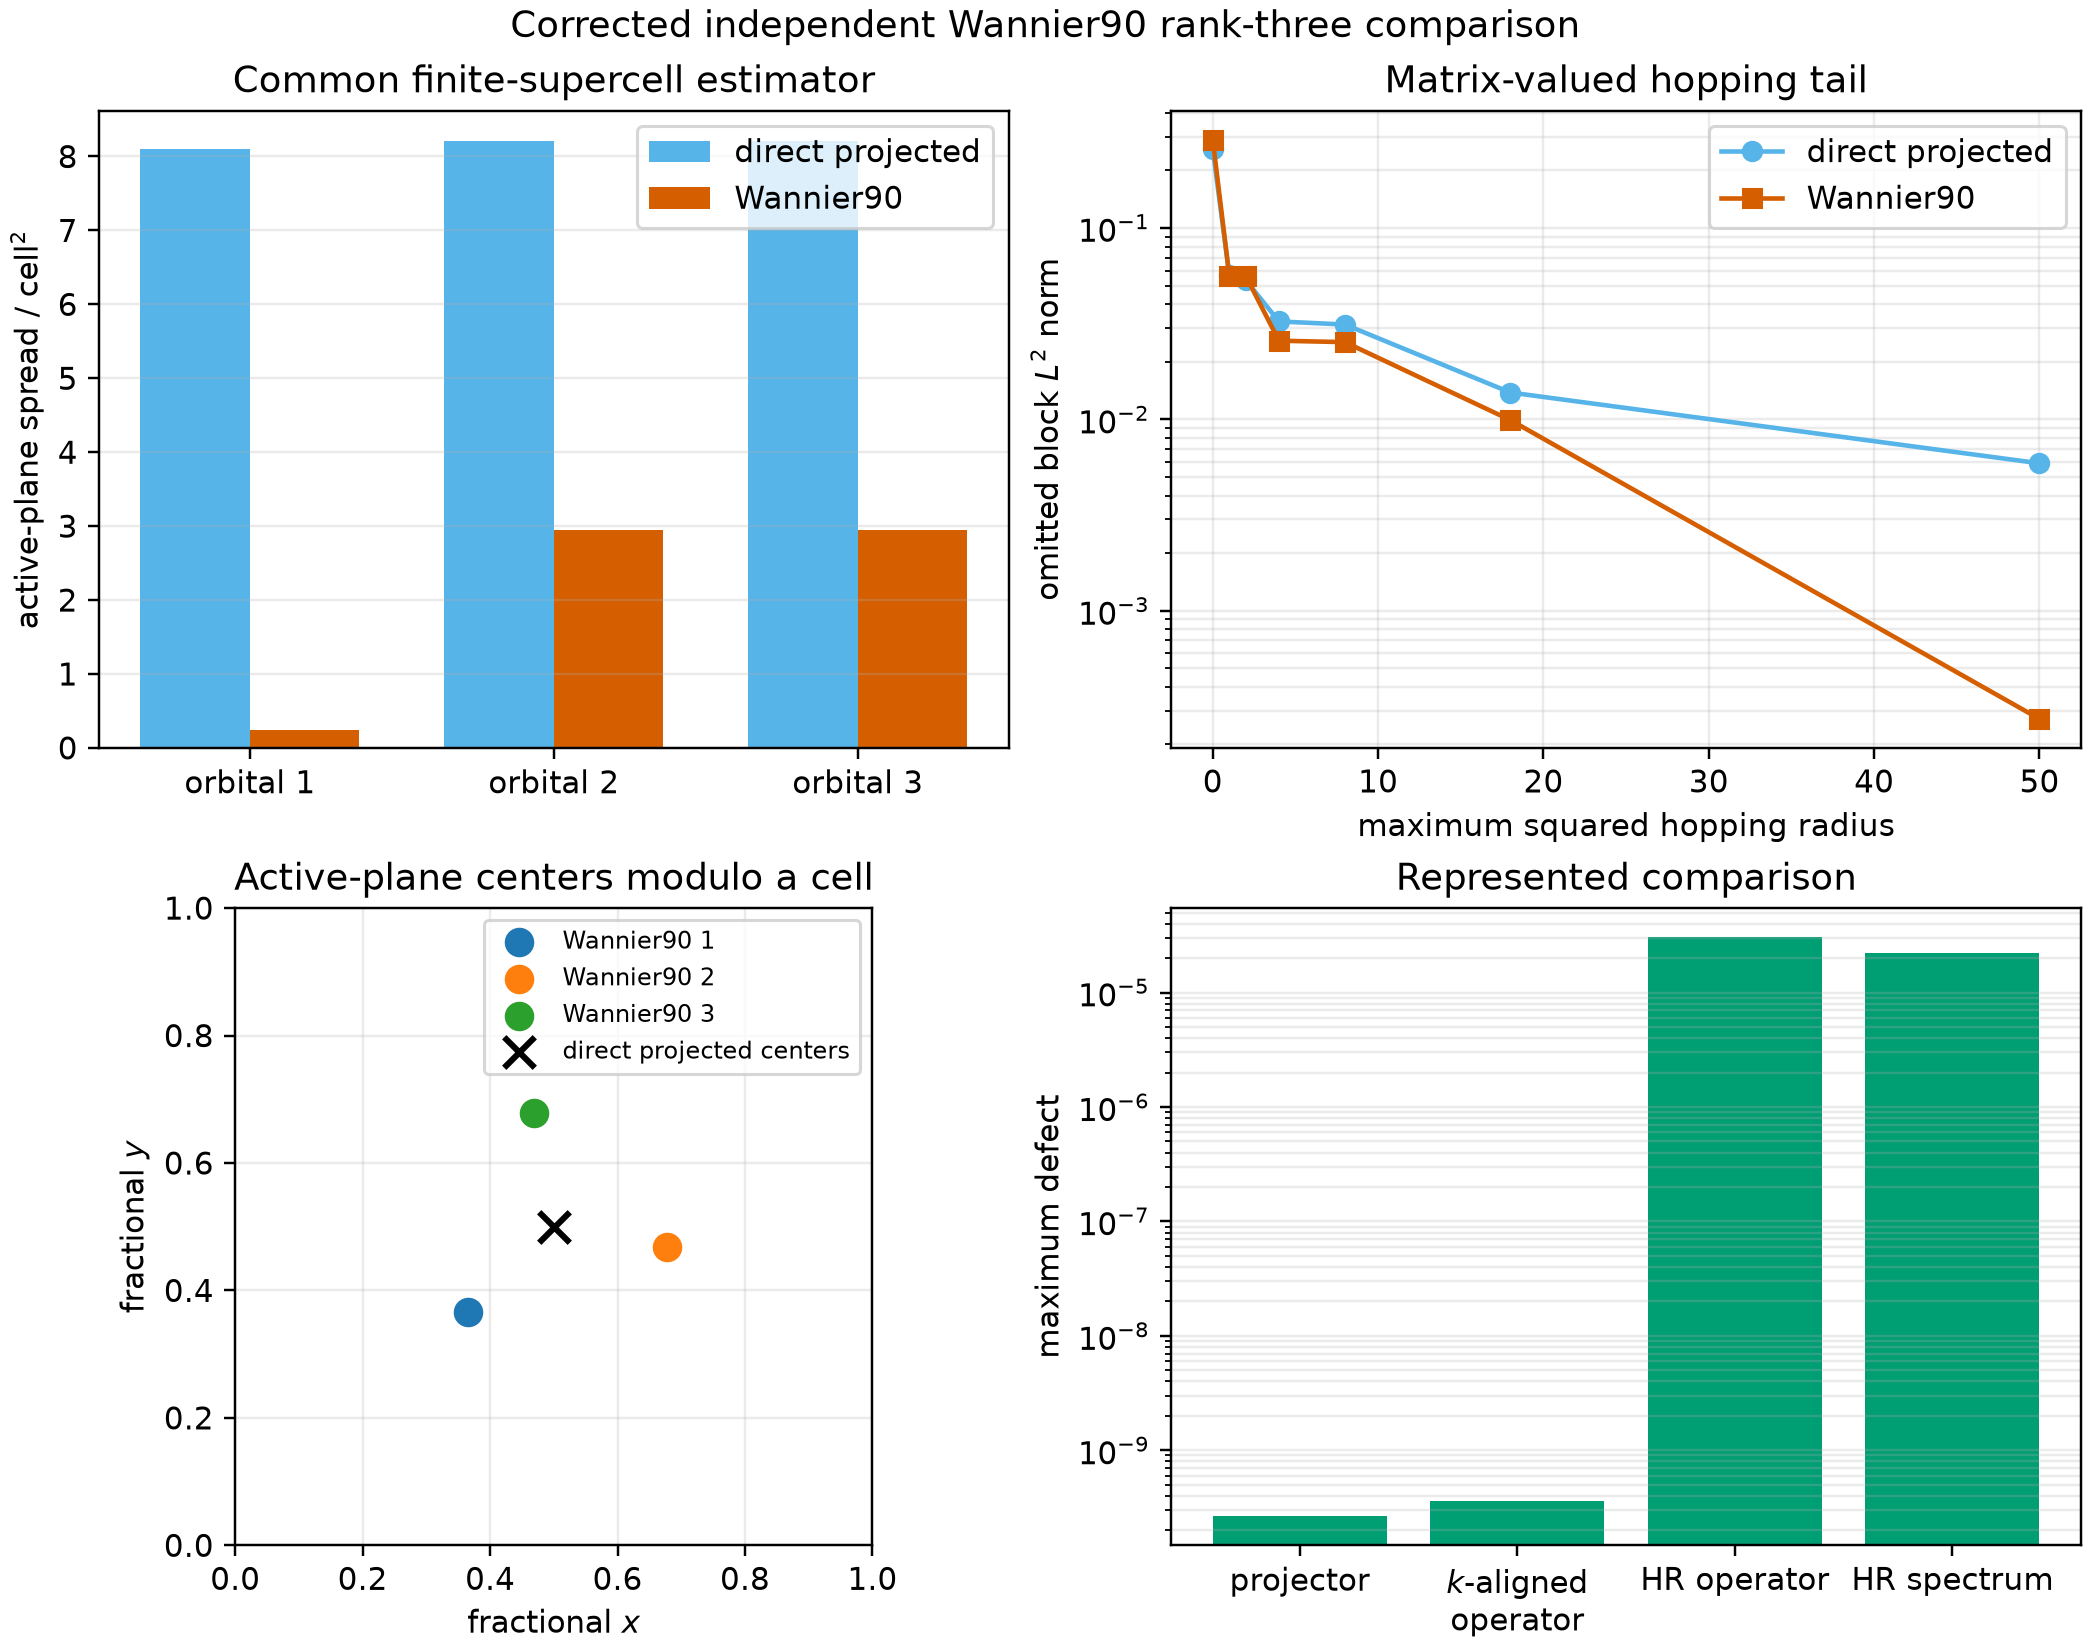
\includegraphics[width=\linewidth,height=0.55\textheight,keepaspectratio]{assets/periodic-2d-wannier90-balanced-summary.png}
    \column{0.37\textwidth}
      \begin{itemize}
        \item Synthetic 2-D, rank-three subspace; no disentanglement.
        \item Projector discrepancy: $2.65\times10^{-10}$.
        \item Pointwise aligned operator discrepancy:
              $3.57\times10^{-10}E_{\mathrm{ref}}$.
        \item Restricted translation/global-unitary family leaves $1.490E_{\mathrm{ref}}$.
        \item Radius-50 tails: $2.72\times10^{-4}E_{\mathrm{ref}}$ and
              $5.90\times10^{-3}E_{\mathrm{ref}}$.
      \end{itemize}
  \end{columns}

  \vspace{0.2em}
  \centering
  One finite algorithm-selected comparison---not global MLWF optimality
  \cite{marzari2012,pizzi2020}.
\end{frame}

\begin{frame}{Periodic DFT still produces Bloch states}
  After self-consistency, a periodic Kohn--Sham operator commutes with lattice
  translations, so its eigenstates may be written
  \cite{kohn1965}
  \[
    \psi_{n\mathbf k}(\mathbf r)
      =e^{i\mathbf k\cdot\mathbf r}u_{n\mathbf k}(\mathbf r),
    \qquad
    u_{n\mathbf k}(\mathbf r)
      =\sum_{\mathbf G}C_{n\mathbf k}(\mathbf G)e^{i\mathbf G\cdot\mathbf r}.
  \]
  \begin{columns}[T]
    \column{0.48\textwidth}
      \begin{block}{What $\mathbf k$ means}
        $\mathbf k$ labels a translation character; $\hbar\mathbf k$ is crystal
        momentum modulo a reciprocal vector. It is not generally an eigenvalue of
        $\hat{\mathbf p}$.
      \end{block}
    \column{0.48\textwidth}
      \begin{block}{What $\hat{\mathbf p}$ means}
        On a plane-wave component,
        \[
          \hat{\mathbf p}\,e^{i(\mathbf k+\mathbf G)\cdot\mathbf r}
          =\hbar(\mathbf k+\mathbf G)e^{i(\mathbf k+\mathbf G)\cdot\mathbf r}.
        \]
        A Bloch state generally contains many such components.
      \end{block}
  \end{columns}

  \centering
  The theorem also accommodates lattice-periodic nonlocal pseudopotential operators;
  it is not restricted to a local scalar potential.
\end{frame}

\begin{frame}{Wavefunction files serialize familiar Bloch states}
  \small
  \begin{columns}[T]
    \column{0.48\textwidth}
      \begin{block}{Typically represented}
        \begin{itemize}
          \item finite-cutoff coefficients $C_{n\mathbf k}(\mathbf G)$;
          \item a finite $\mathbf k$ mesh, bands, spins or spinors;
          \item eigenvalues, occupations, and implementation metadata.
        \end{itemize}
        VASP calls one such file \texttt{WAVECAR}; Quantum ESPRESSO uses implementation-
        specific wavefunction files such as \texttt{.wfc*}.
      \end{block}
    \column{0.48\textwidth}
      \begin{alertblock}{Not fixed by that file alone}
        \begin{itemize}
          \item a canonical band phase or multiband gauge;
          \item a Wannier subspace or localization choice;
          \item the full self-consistent density and potential;
          \item pseudopotential/PAW augmentation data;
          \item energy-reference and provenance contracts.
        \end{itemize}
      \end{alertblock}
  \end{columns}

  \[
    \text{wavefunction files + companion data}
    \rightarrow \{\psi_{n\mathbf k}\}
    \rightarrow \text{subspace/projectors}
    \rightarrow U(\mathbf k)
    \rightarrow \text{Wannier/TB blocks}.
  \]
  The gauge step is essential: within an isolated or selected subspace,
  $\psi_{n\mathbf k}\mapsto\sum_m\psi_{m\mathbf k}U_{mn}(\mathbf k)$ preserves the
  represented subspace but can change locality \cite{marzari2012,pizzi2020}.
\end{frame}

\begin{frame}{Wannier transformation: a localized operator representation}
  \small
  For a selected rank-$r$ Bloch subspace and gauge $U(\mathbf k)$,
  \[
    |\mathbf R n\rangle
      =\frac{1}{\sqrt{N_k}}\sum_{\mathbf k}e^{-i\mathbf k\cdot\mathbf R}
       \sum_{m=1}^{r}|\psi_{m\mathbf k}\rangle U_{mn}(\mathbf k).
  \]
  A translation-covariant operator is represented by real-space blocks
  \[
    O^W_{mn}(\mathbf R)
      =\langle\mathbf 0m|\hat O|\mathbf Rn\rangle
      =\frac{1}{N_k}\sum_{\mathbf k}e^{-i\mathbf k\cdot\mathbf R}
       \bigl[U^\dagger(\mathbf k)O(\mathbf k)U(\mathbf k)\bigr]_{mn}.
  \]
  \begin{columns}[T]
    \column{0.48\textwidth}
      \begin{block}{What localization can provide}
        A nonlocal operator kernel can have rapidly decaying matrix elements in a
        localized Wannier basis. This exposes a physically useful local representation
        and possible finite-range compression.
      \end{block}
    \column{0.48\textwidth}
      \begin{alertblock}{What it does not guarantee}
        The operator has not become local as an abstract operator, and its Wannier
        blocks need not have finite support. Decay depends on the subspace, gauge,
        regularity, gaps, and possible topological obstruction.
      \end{alertblock}
  \end{columns}

  \centering
  Eigenvalues plus $U(\mathbf k)$ determine the projected Hamiltonian; kinetic,
  pseudopotential, and other components require their own same-frame matrix elements.
\end{frame}

\begin{frame}{Result 4: silicon tutorial operators in one common frame}
  \begin{align*}
    W(\mathbf k)&=U_{\mathrm{dis}}(\mathbf k)U(\mathbf k),\\
    \HW(\mathbf k)&=W^\dagger\operatorname{diag}(\epsilon)W,\\
    \TW(\mathbf k)&=W^\dagger C_{\mathrm{PW}}^\dagger
    \operatorname{diag}\!\left(\frac{|\mathbf k+\mathbf G|^2}{2}\right)
    C_{\mathrm{PW}}W,\\
    \RW(\mathbf k)&=\HW(\mathbf k)-\TW(\mathbf k).
  \end{align*}

  \begin{columns}[T]
    \column{0.51\textwidth}
      \begin{block}{Finite checks}
        Same-frame subtraction discrepancy: $1.52\times10^{-15}$ eV.\\
        Native \texttt{\_hr.dat} route difference: $1.28\times10^{-5}$ eV.
      \end{block}
    \column{0.45\textwidth}
      \begin{alertblock}{Boundary}
        QE 7.5/Wannier90 3.1.0 tutorial, 25 Ry, 12 bands, four Wannier functions,
        $4^3$ mesh. Not a converged production silicon model.
      \end{alertblock}
  \end{columns}
\end{frame}

\begin{frame}{Result 4a: component block distributions differ}
  \begin{center}
    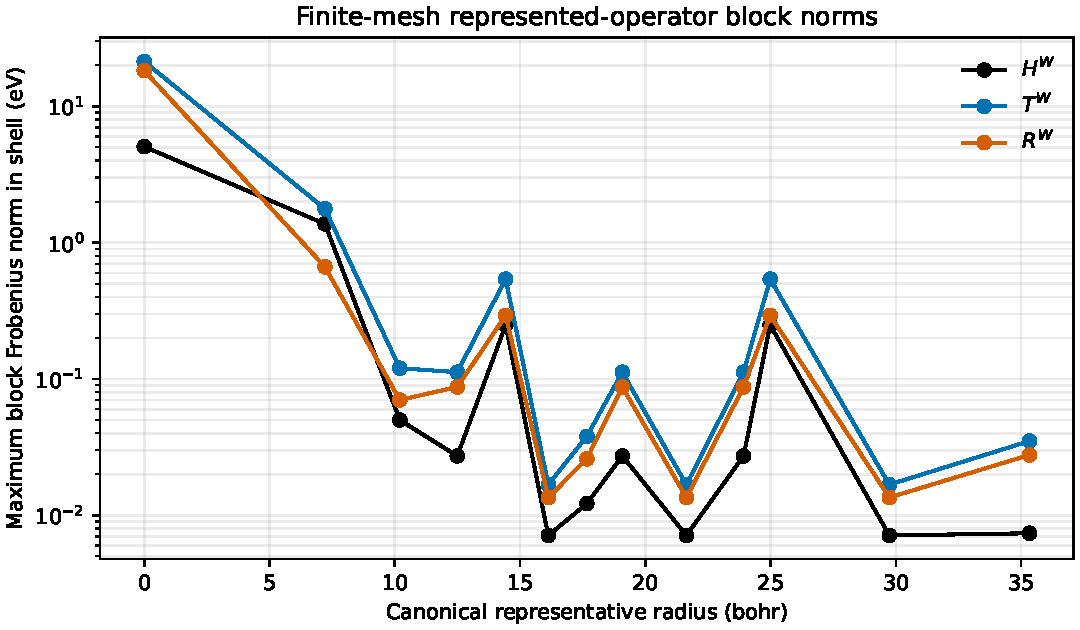
\includegraphics[width=0.72\textwidth,height=0.57\textheight,keepaspectratio]{assets/silicon-real-space-shell-block-norms.pdf}
  \end{center}
  \vspace{-0.7em}
  \begin{itemize}
    \item At every nonzero represented radius, the maximum kinetic block exceeds the
          maximum remainder block by approximately $1.24$--$2.67$.
    \item Cancellation can make the total block smaller than either component.
    \item Sixty-four nonmonotone blocks do not determine an infinite-lattice decay law.
  \end{itemize}
\end{frame}

\begin{frame}{Result 4b: 57-block truncation is not component-neutral}
  \begin{columns}[T]
    \column{0.62\textwidth}
      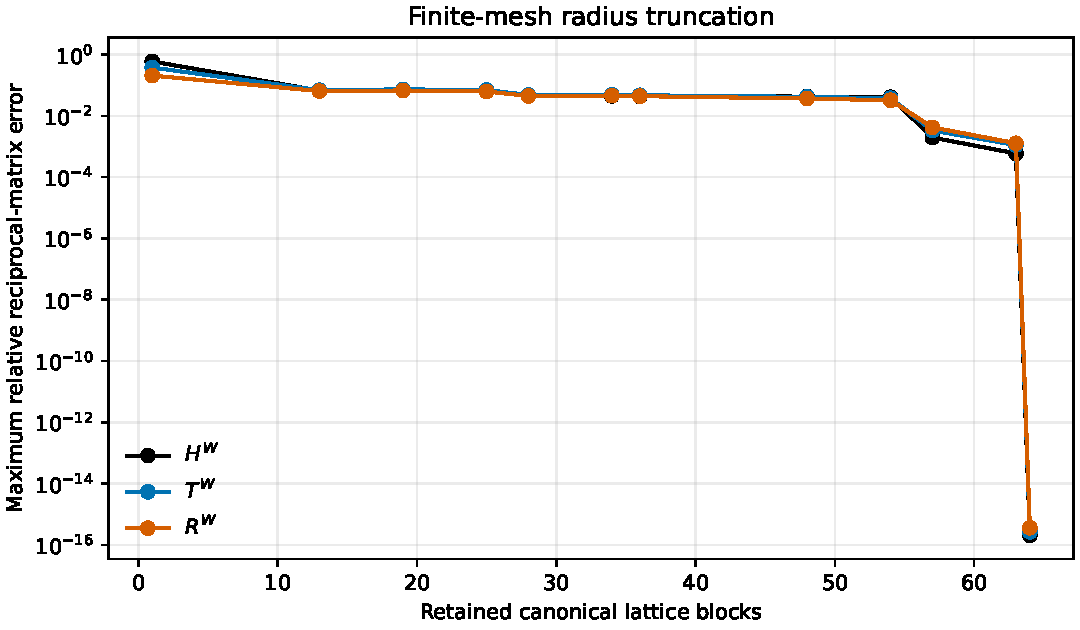
\includegraphics[width=\linewidth]{assets/silicon-real-space-truncation-relative-error.pdf}
    \column{0.35\textwidth}
      \begin{block}{Maximum band error}
        \centering
        \begin{tabular}{lc}
          \toprule
          Component & 57/64 blocks\\
          \midrule
          $\HW$ & 20.7 meV\\
          $\TW$ & 84.3 meV\\
          $\RW$ & 63.6 meV\\
          \bottomrule
        \end{tabular}
      \end{block}
      \vspace{0.5em}
      All 64 blocks recover the sampled matrices to roundoff.
  \end{columns}

  \vspace{0.3em}
  \centering
  Failure of one finite-mesh truncation $\neq$ failure of tight binding generally.
\end{frame}

\begin{frame}{What the four results establish together}
  \small
  \begin{tabular}{p{0.15\textwidth}p{0.35\textwidth}p{0.39\textwidth}}
    \toprule
    Stage & Established & Not established\\
    \midrule
    Rank-two 1-D & Exact band equivalence with sampled range inflation & Universal range law\\
    Scalar 2-D & Separation of tensor reconstruction, mixed coupling, and interpolation & 3-D or non-orthogonal outcome\\
    Rank-three 2-D & Gauge-consistent spectra with different finite locality diagnostics & Global localization optimum or topology\\
    Silicon tutorial & Same-frame decomposition and failure of one component truncation & Production silicon adequacy\\
    \bottomrule
  \end{tabular}

  \vspace{0.8em}
  \begin{block}{Common methodological conclusion}
    Complete fields, eigenvalues, projector/frame choices, Fourier conversion, and
    finite-range truncation must be kept as distinct information channels.
  \end{block}
\end{frame}

\begin{frame}{Two-axis validation ladder}
  \centering
  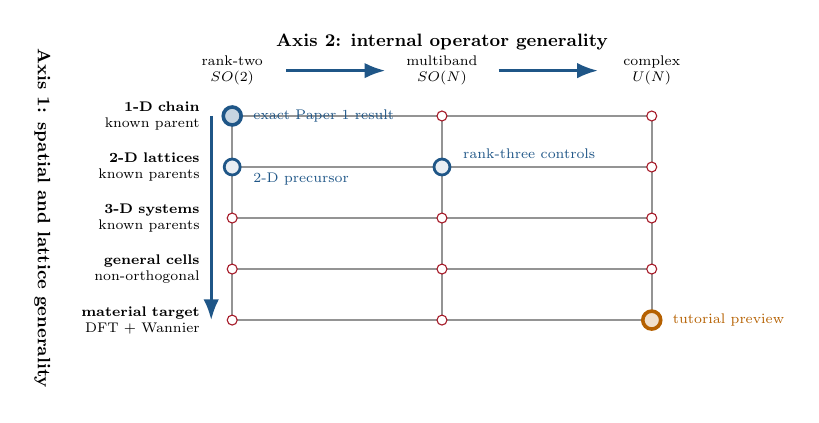
\begin{tikzpicture}[
    >=Latex,scale=0.72,transform shape,
    gridline/.style={line width=0.75pt,black!42},
    progression/.style={->,line width=1pt,resultblue},
    stage/.style={font=\scriptsize,align=right,text width=2.55cm},
    column/.style={font=\scriptsize,align=center,text width=2.7cm},
    empty/.style={circle,draw=prospectivered,fill=white,minimum size=5pt,inner sep=0pt},
    established/.style={circle,draw=resultblue,line width=1.3pt,fill=resultblue!25,
                        minimum size=9pt,inner sep=0pt},
    bounded/.style={circle,draw=resultblue,line width=1pt,fill=resultblue!10,
                    minimum size=8pt,inner sep=0pt},
    preview/.style={circle,draw=previeworange,line width=1.3pt,fill=previeworange!20,
                    minimum size=9pt,inner sep=0pt}
  ]
    \node[font=\small\bfseries] at (5.0,4.85)
      {Axis 2: internal operator generality};
    \node[font=\small\bfseries,rotate=270] at (-2.05,1.75)
      {Axis 1: spatial and lattice generality};
    \node[column] at (1.3,4.35) {rank-two\\$SO(2)$};
    \node[column] at (5.0,4.35) {multiband\\$SO(N)$};
    \node[column] at (8.7,4.35) {complex\\$U(N)$};
    \draw[progression] (2.25,4.35) -- (4.0,4.35);
    \draw[progression] (6.0,4.35) -- (7.75,4.35);

    \node[stage] at (-0.55,3.55) {\textbf{1-D chain}\\known parent};
    \node[stage] at (-0.55,2.65) {\textbf{2-D lattices}\\known parents};
    \node[stage] at (-0.55,1.75) {\textbf{3-D systems}\\known parents};
    \node[stage] at (-0.55,0.85) {\textbf{general cells}\\non-orthogonal};
    \node[stage] at (-0.55,-0.05) {\textbf{material target}\\DFT + Wannier};

    \foreach \y in {-0.05,0.85,1.75,2.65,3.55}
      \draw[gridline] (1.3,\y) -- (8.7,\y);
    \foreach \x in {1.3,5.0,8.7}
      \draw[gridline] (\x,-0.05) -- (\x,3.55);
    \draw[progression] (0.93,3.55) -- (0.93,-0.05);
    \foreach \x in {1.3,5.0,8.7}
      \foreach \y in {-0.05,0.85,1.75,2.65,3.55}
        \node[empty] at (\x,\y) {};

    \node[established] at (1.3,3.55) {};
    \node[bounded] at (1.3,2.65) {};
    \node[bounded] at (5.0,2.65) {};
    \node[preview] at (8.7,-0.05) {};

    \node[font=\scriptsize,resultblue,anchor=west] at (1.55,3.55)
      {exact Paper 1 result};
    \node[font=\scriptsize,resultblue,anchor=west] at (1.55,2.43)
      {2-D precursor};
    \node[font=\scriptsize,resultblue,anchor=west] at (5.25,2.88)
      {rank-three controls};
    \node[font=\scriptsize,previeworange,anchor=west] at (8.95,-0.05)
      {tutorial preview};

  \end{tikzpicture}

  \vspace{-0.3em}
  \begin{columns}[T]
    \column{0.58\textwidth}
      \small
      \textcolor{resultblue}{Filled blue: established or bounded controlled evidence.}
      \textcolor{previeworange}{Orange: bounded tutorial preview.}
    \column{0.38\textwidth}
      \small\future{Red outlines: prospective experiments, not results.}
  \end{columns}

  \vfill
  \centering
  This map separates accumulated bounded evidence from the unexecuted validation
  roadmap.
\end{frame}

\begin{frame}{Why bulk compatibility matters for the Si:P objective}
  \begin{enumerate}
    \item \textbf{Band equivalence does not determine hopping locality.}
    \item \textbf{The desired Si:P perturbation is a difference of aligned operators,}
          not a difference of band energies or independently gauged Wannier files.
    \item \textbf{Projection, gauge selection, Fourier conversion, interpolation, and
          deliberate truncation preserve different information.}
    \item \textbf{Equal sampled accuracy---not equal cutoff---is the meaningful
          representation-cost comparison.}
    \item \textbf{The silicon tutorial establishes failure of one component-wise
          finite-mesh truncation, not failure of tight binding generally.}
  \end{enumerate}

  \vfill
  \centering
  \future{Next ICMSEP production step: a qualified bulk-Si parent, validated Wannier
  operator, and frozen compatibility search. Si:P follows only after that reference is
  accepted.}\\[0.65em]
  
\includegraphics[width=.25\textwidth]{assets/dlsu-wordmark-green.png}\\[0.35em]
  \Large Thank you
\end{frame}

\begin{frame}[noframenumbering]{References}
  \printbibliography[heading=none]
\end{frame}

\end{document}
